%!TEX root = prelim.tex

\subsection{Acquisition System}
\frame{
\frametitle{Training Rig Background}
\begin{columns}

\begin{column}{0.7\textwidth}
Traditional Flash-Based system
\begin{itemize}
\item Used for most public data sets
\item Difficult to reconfigure
\item Does not scale well in the number of flashes
\item Need room sized dome for good angular coverage, distant illumination
\end{itemize}
Projector-Based system
\begin{itemize}
\item Easy to re-configure projector geometry
\item Trivial to change illumination patterns
\item Easier to construct and deploy
\item Very complete angular illumination coverage
\end{itemize}
\end{column}

\begin{column}{0.3\textwidth}
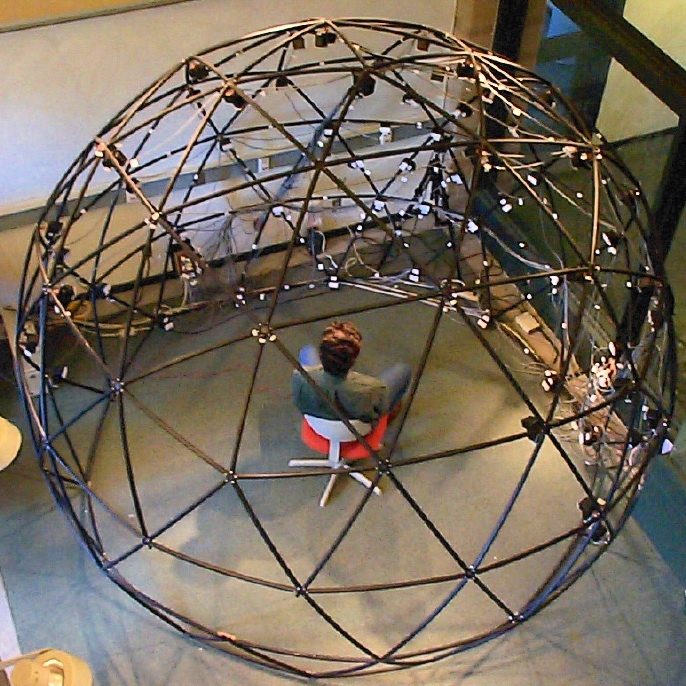
\includegraphics[width=\textwidth]{images/yale_dome.jpg}\\ 
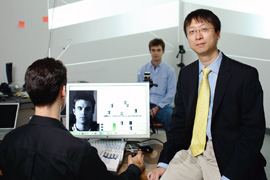
\includegraphics[width=\textwidth]{images/projector_photo.jpg} \\ \vspace{0\textheight}
\end{column}
\end{columns}
}

\frame{
\frametitle{Training Illumination Rig}
\begin{center}
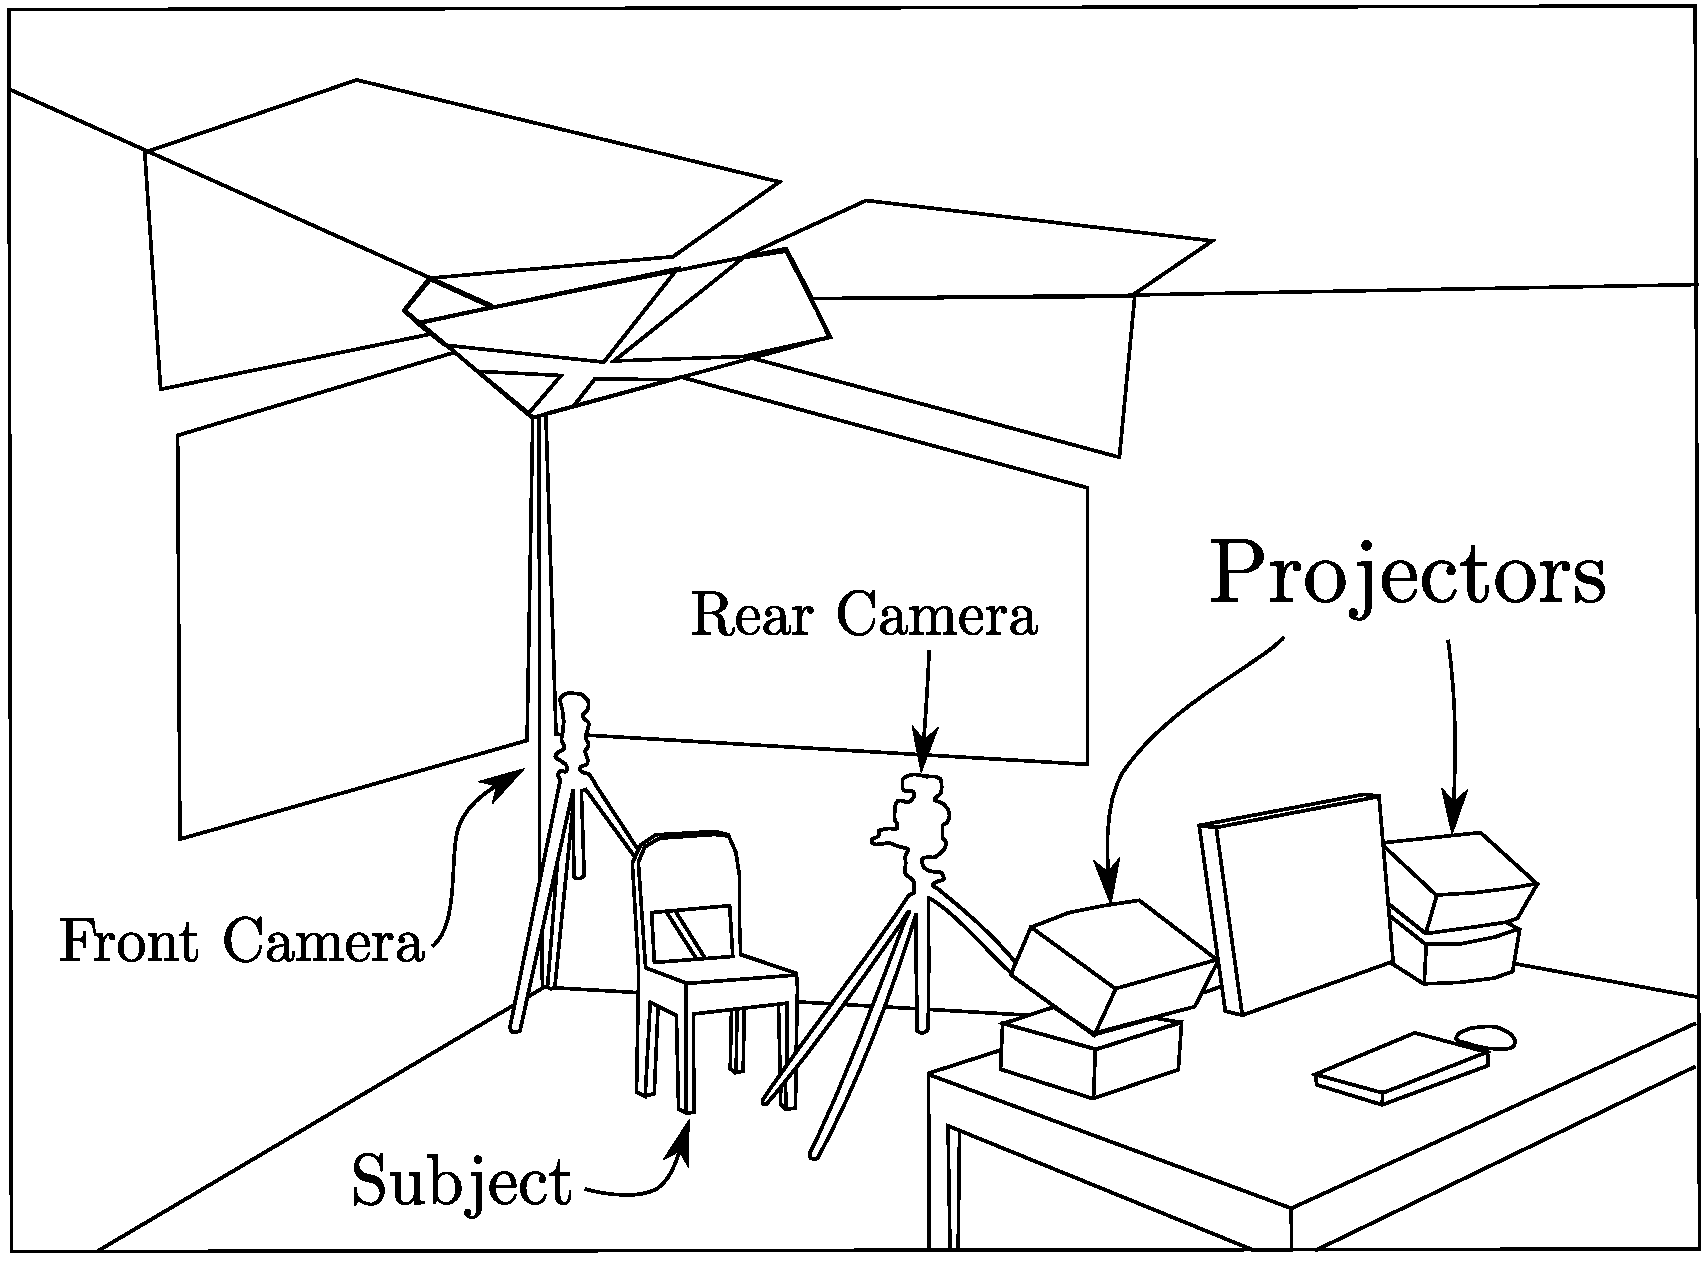
\includegraphics[width=0.8\textwidth]{images/camera_rig_drawings/perspective.pdf}
\end{center}
}

\frame{
\frametitle{Training Illumination Rig}
\begin{columns}
\begin{column}{.5\textwidth}
\begin{center}
Side View\\
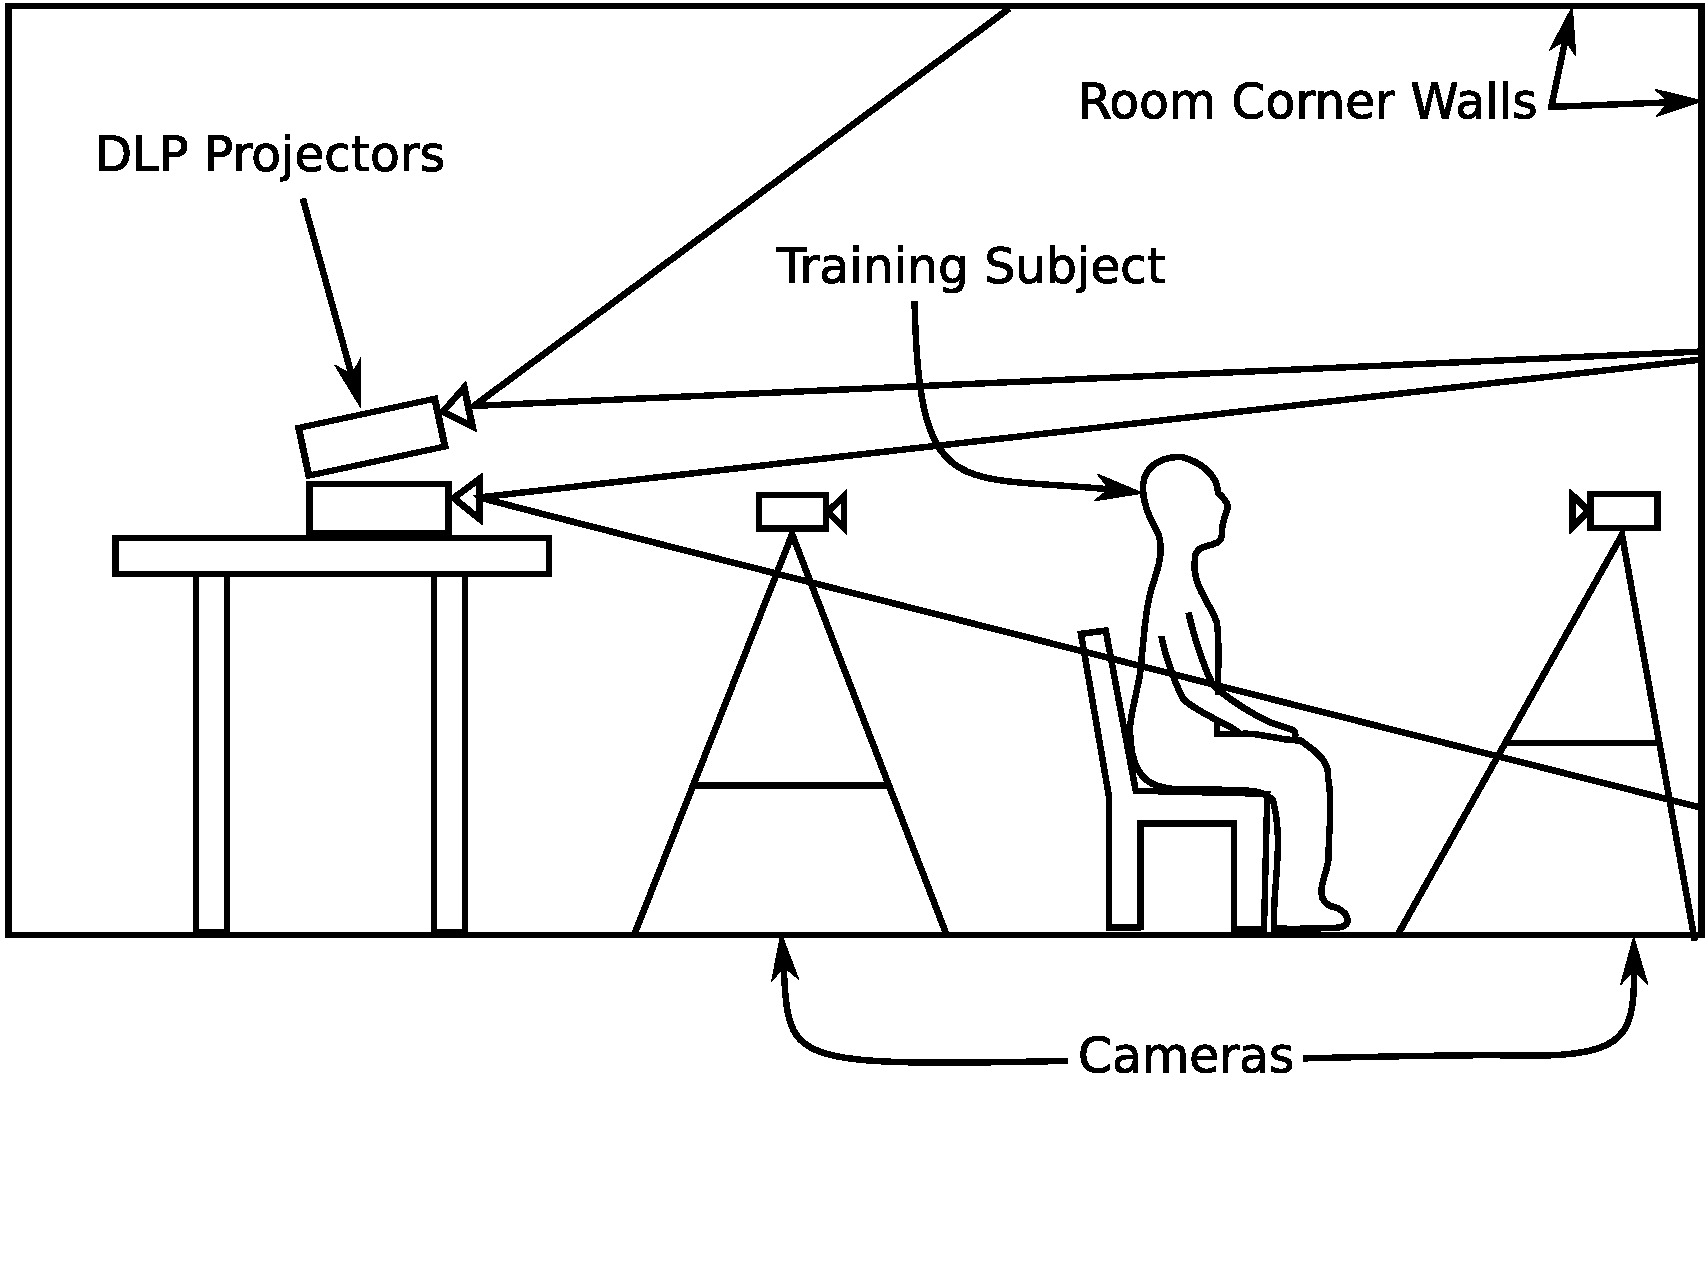
\includegraphics[width=\textwidth]{images/camera_rig_drawings/coverage_side.pdf}
\end{center}
\end{column}
\begin{column}{.5\textwidth}
\begin{center}
Top View\\
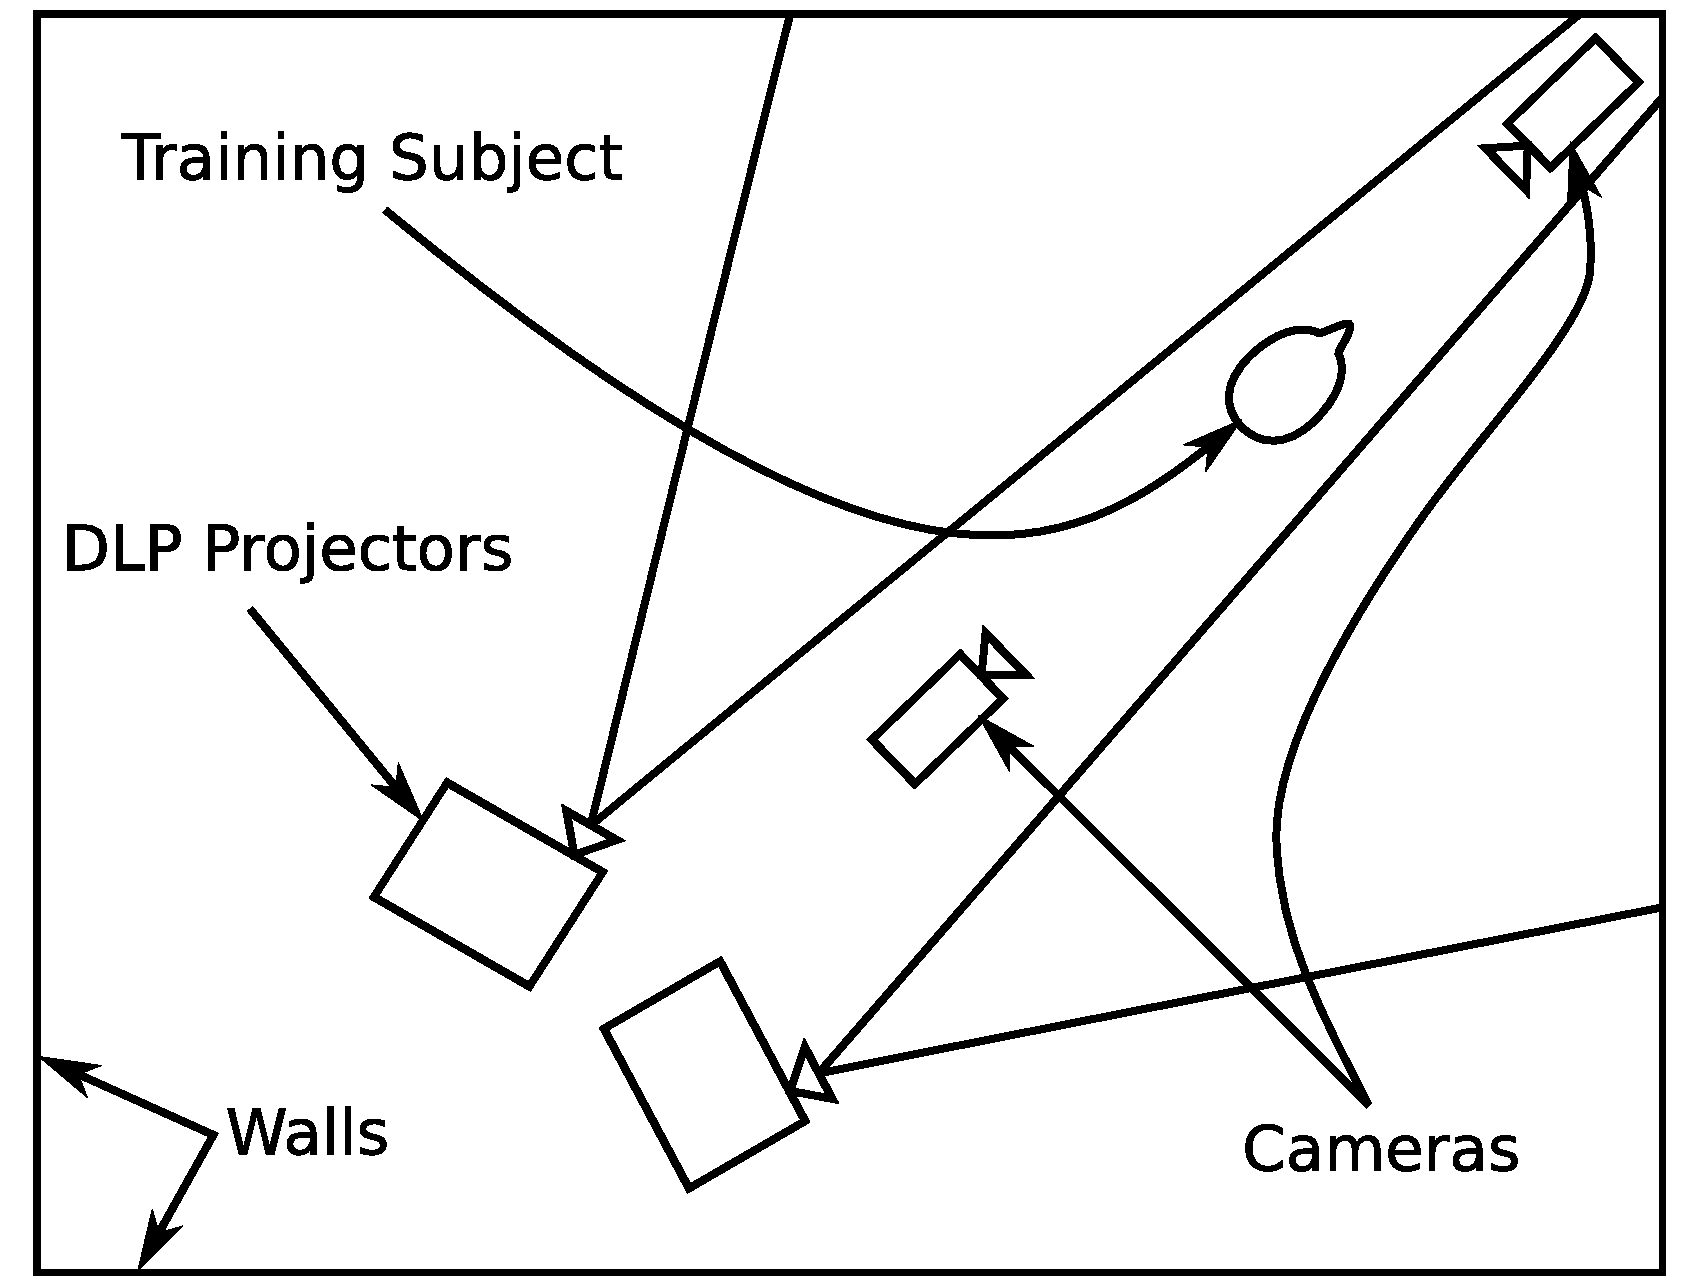
\includegraphics[width=\textwidth]{images/camera_rig_drawings/coverage_top.pdf}
\end{center}
\end{column}
\end{columns}
}

\frame{
\frametitle{So many projector pixels, so little time}
\begin{itemize}
\item Need to narrow down the illumination possibilities.
\item How densely do we need to sample the illumination sphere?
\begin{itemize}
\item Try multiple sets of illuminations
\item Double the resolution in one direction each time
\end{itemize}
\item How much coverage do we need?
\begin{itemize}
\item Try multiple sets of illuminations
\item Gradually increase the coverage radially out from known-important illuminations
\end{itemize}
\end{itemize}
\begin{center}
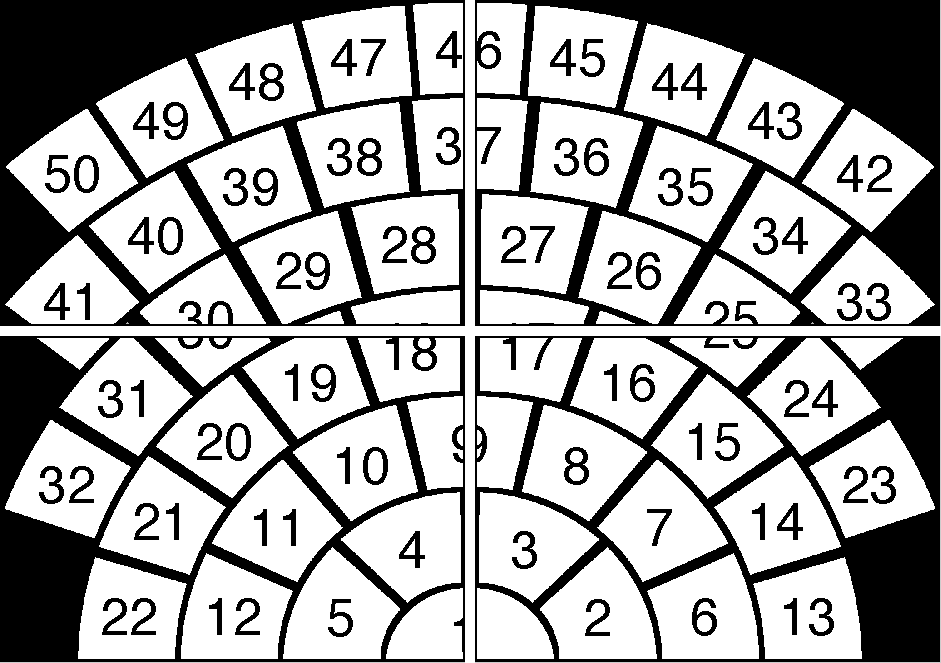
\includegraphics[height=.4\textheight]{figures_cvpr/coverage_experiment_asplode_white.png}
\end{center}
}

\renewcommand{\imagesizestring}{height}
\frame{\frametitle{Illumination Experiment Results}
\renewcommand{\imagesizea}{0.55\textheight}
\begin{center}
\begin{tabular}{cc}
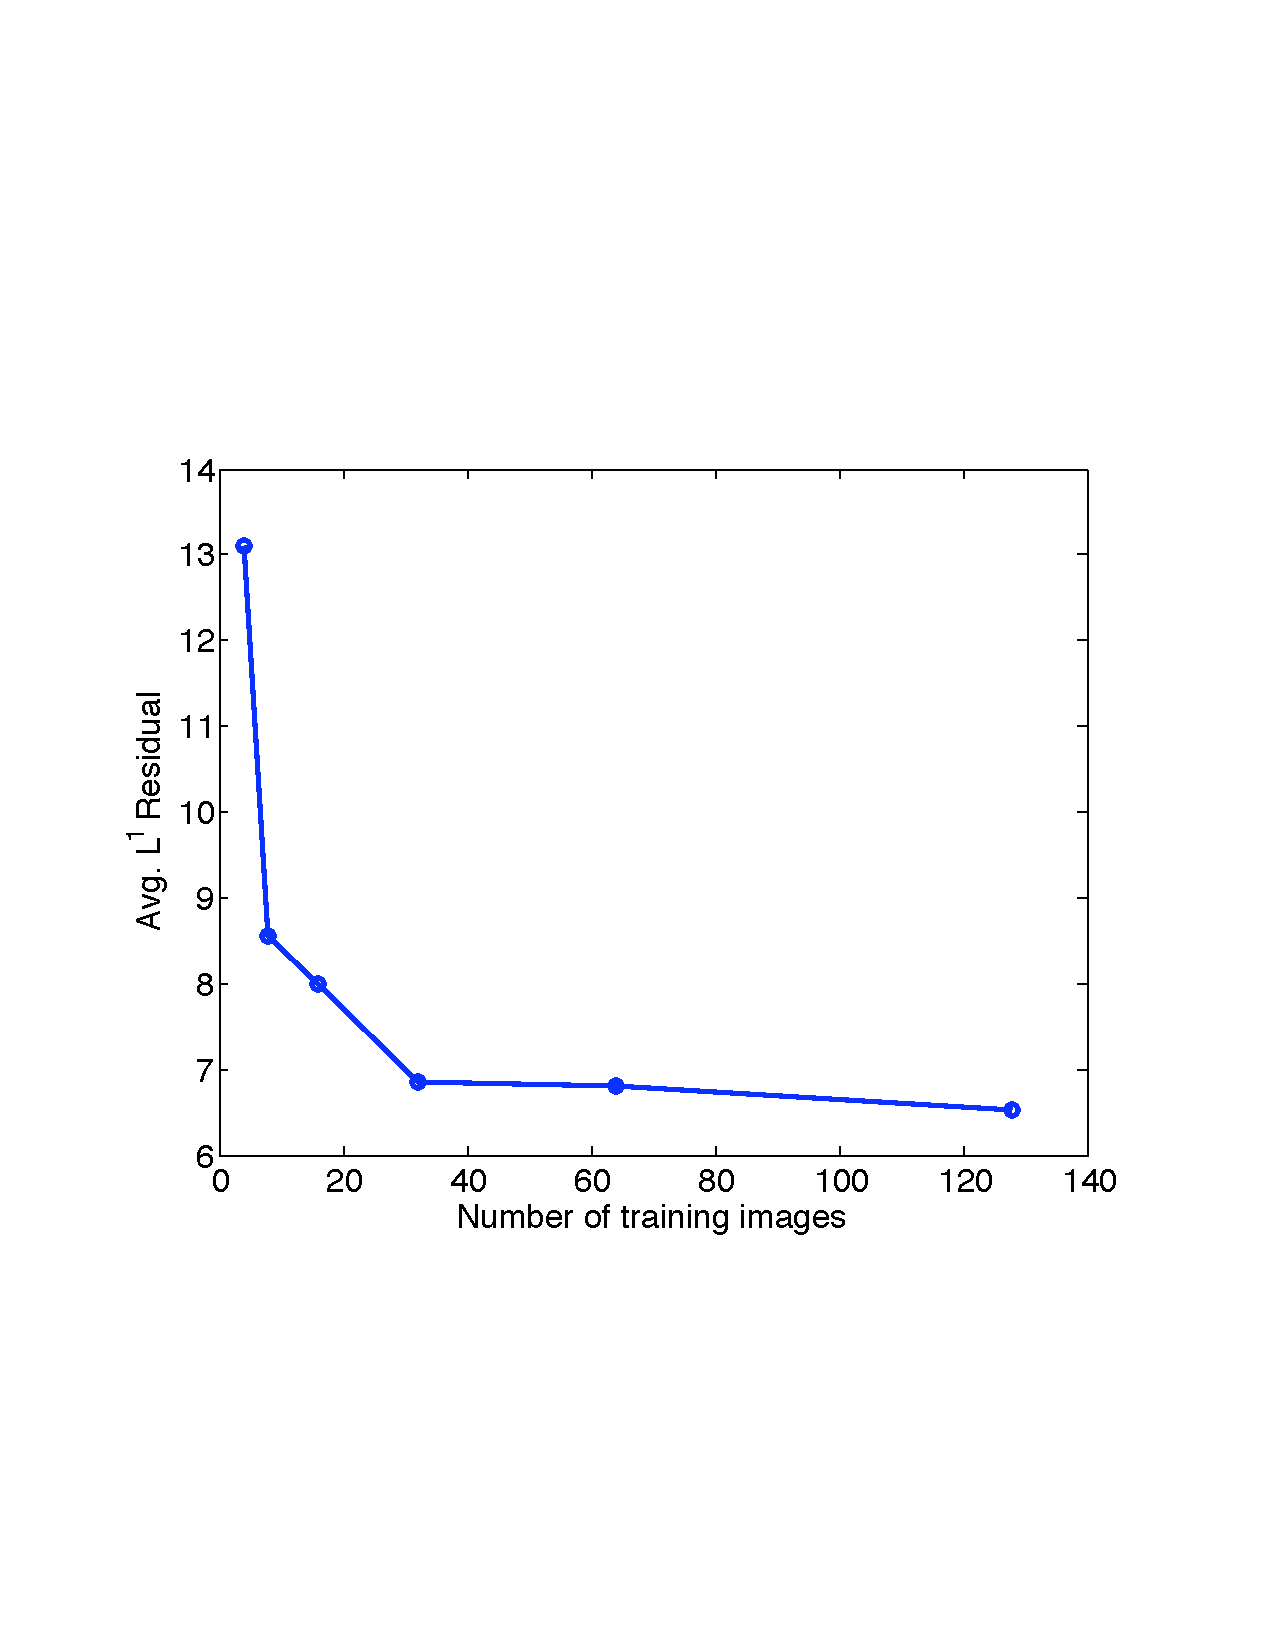
\includegraphics[\imagesizestring=\imagesizea]{figures_cvpr/illum_results/granularity_sunset.pdf} &
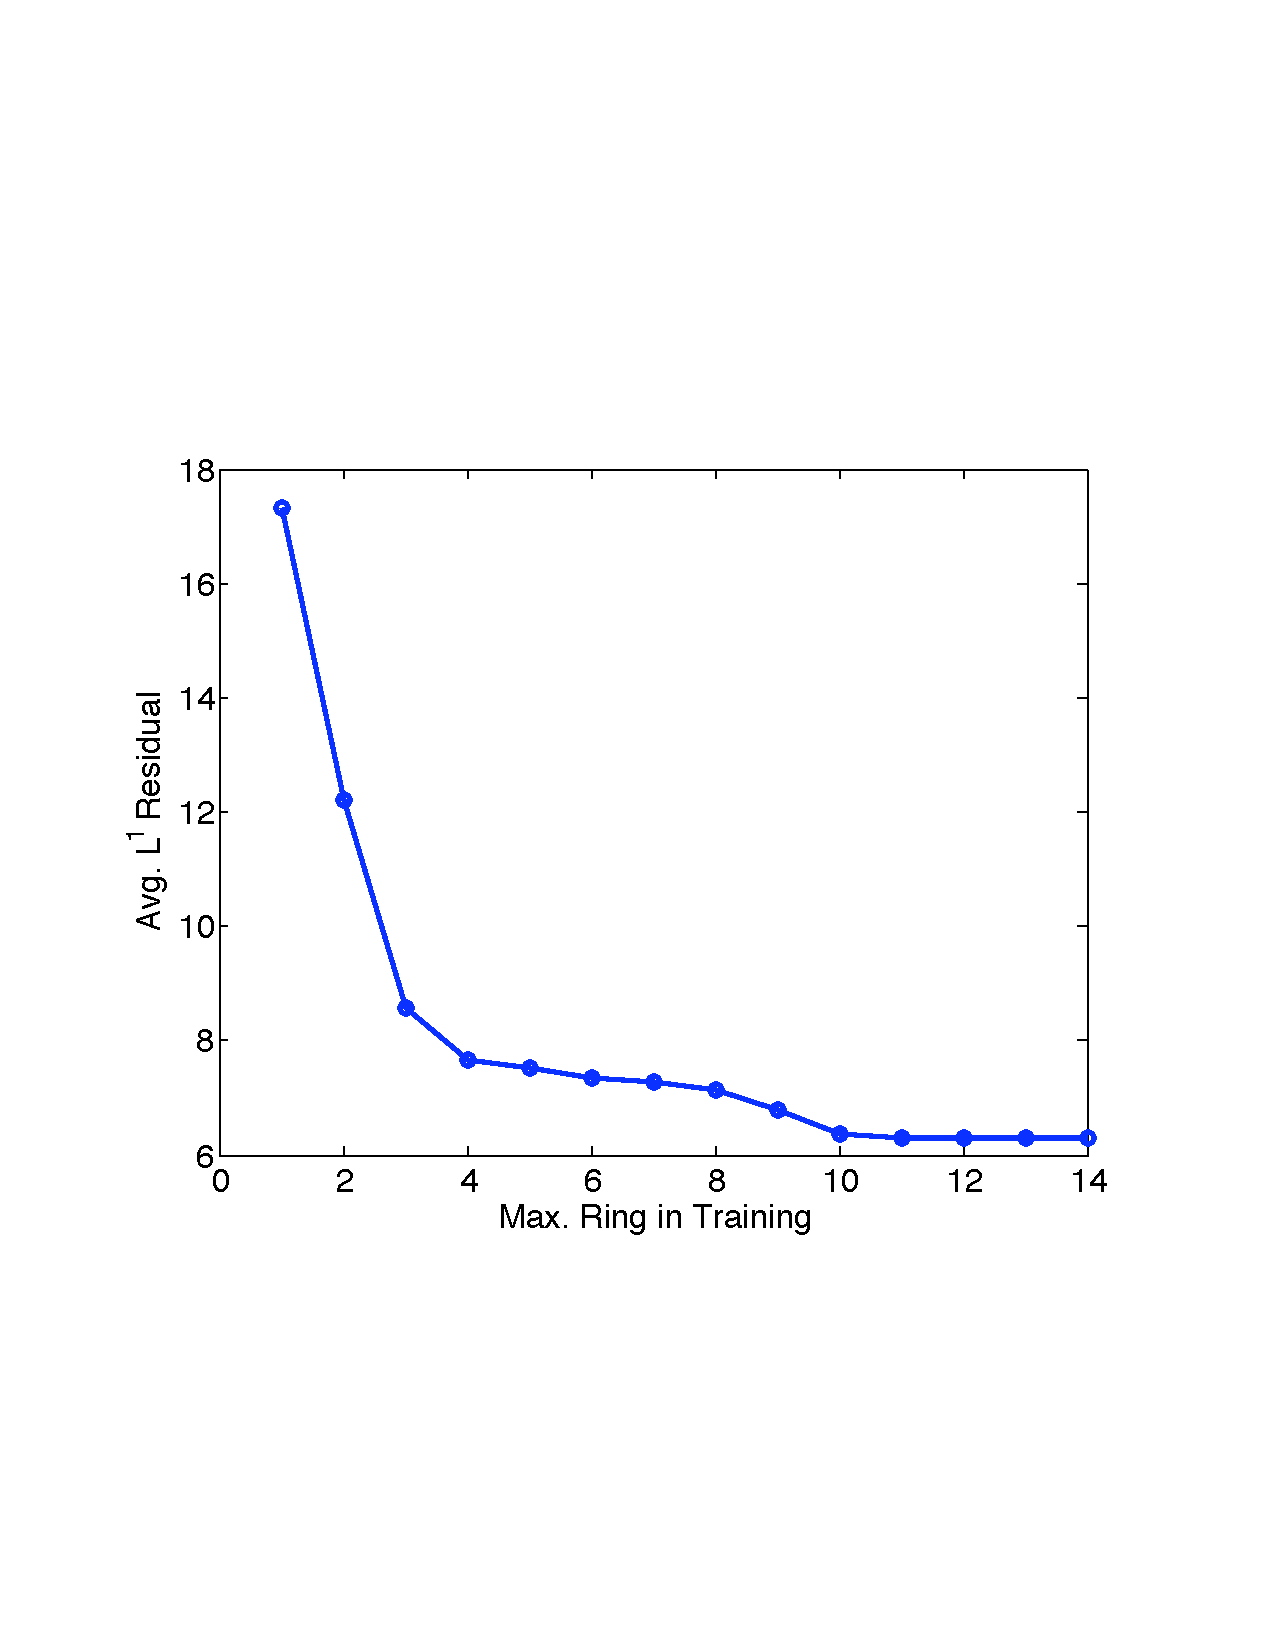
\includegraphics[\imagesizestring=\imagesizea]{figures_cvpr/illum_results/coverage_sunset.pdf} \\
(a) Granularity & (b) Coverage
\end{tabular}\vspace{2mm}
\end{center}
}

\frame{
\renewcommand{\imagesizestring}{height}
\renewcommand{\imagesizea}{0.41\textheight}
\frametitle{Final Illuminations}
\begin{tabular}{cc}
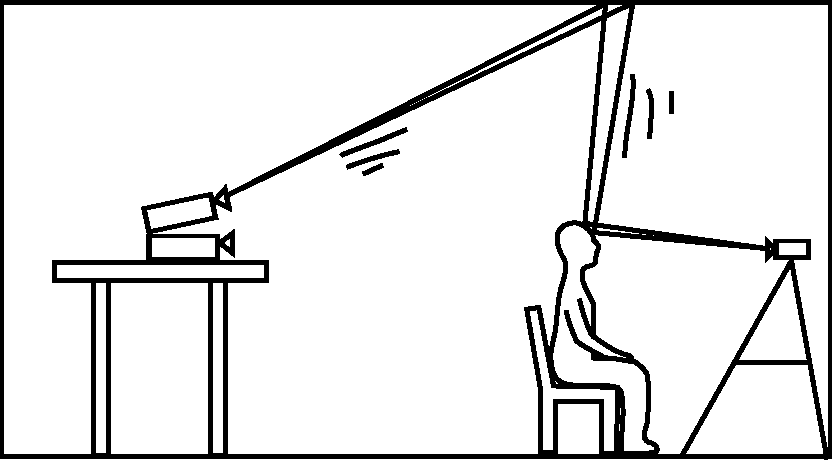
\includegraphics[\imagesizestring = \imagesizea]{images/camera_rig_drawings/side_front.pdf} & 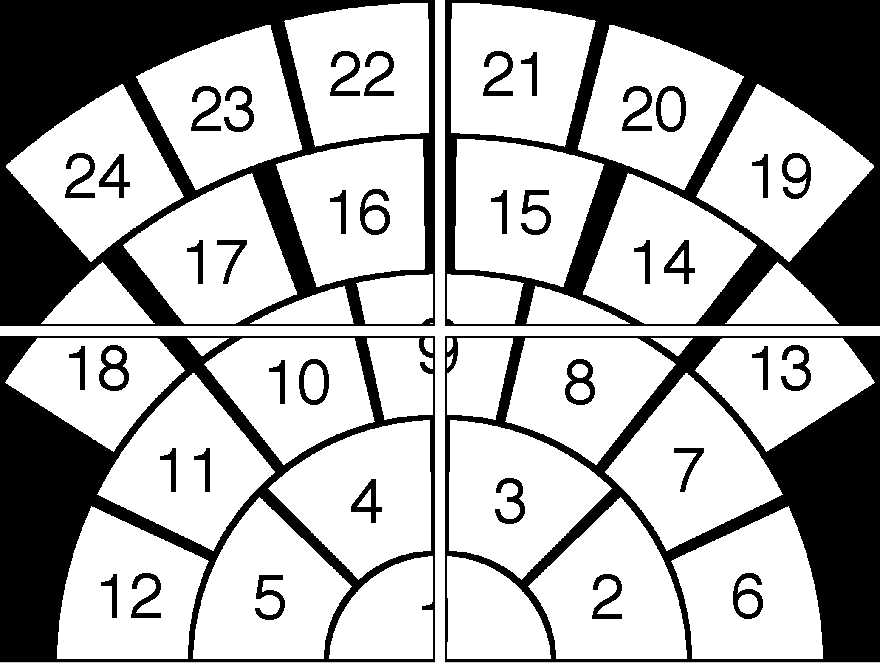
\includegraphics[\imagesizestring = \imagesizea]{images/illuminations/front.png}\\
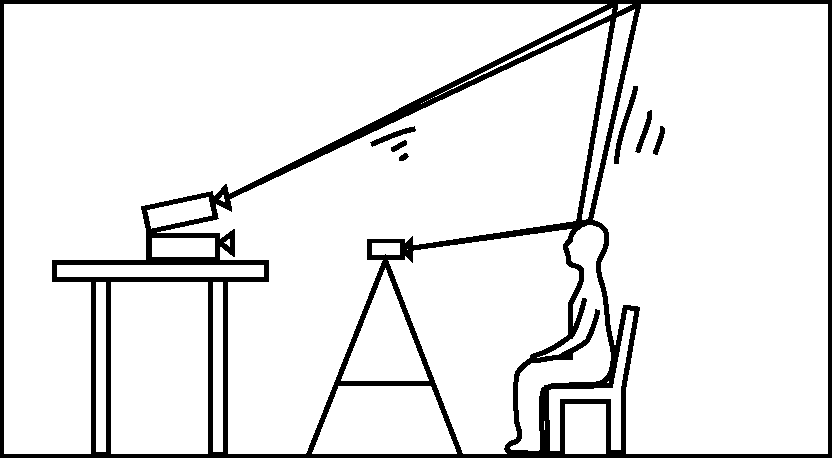
\includegraphics[\imagesizestring = \imagesizea]{images/camera_rig_drawings/side_back.pdf} & 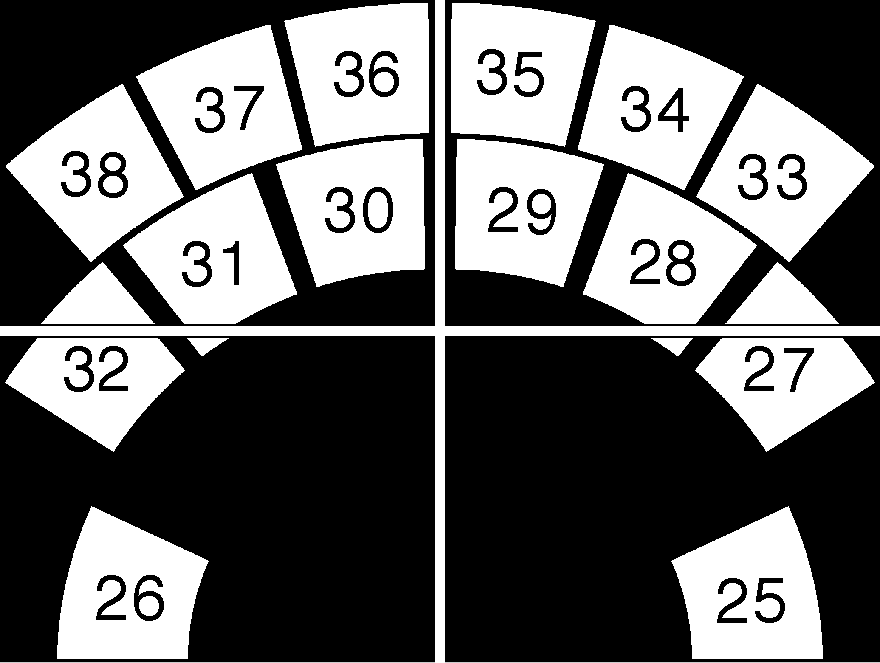
\includegraphics[\imagesizestring = \imagesizea]{images/illuminations/back.png}
\end{tabular}
}


\frame{\frametitle{Sample Training Images, Originals}
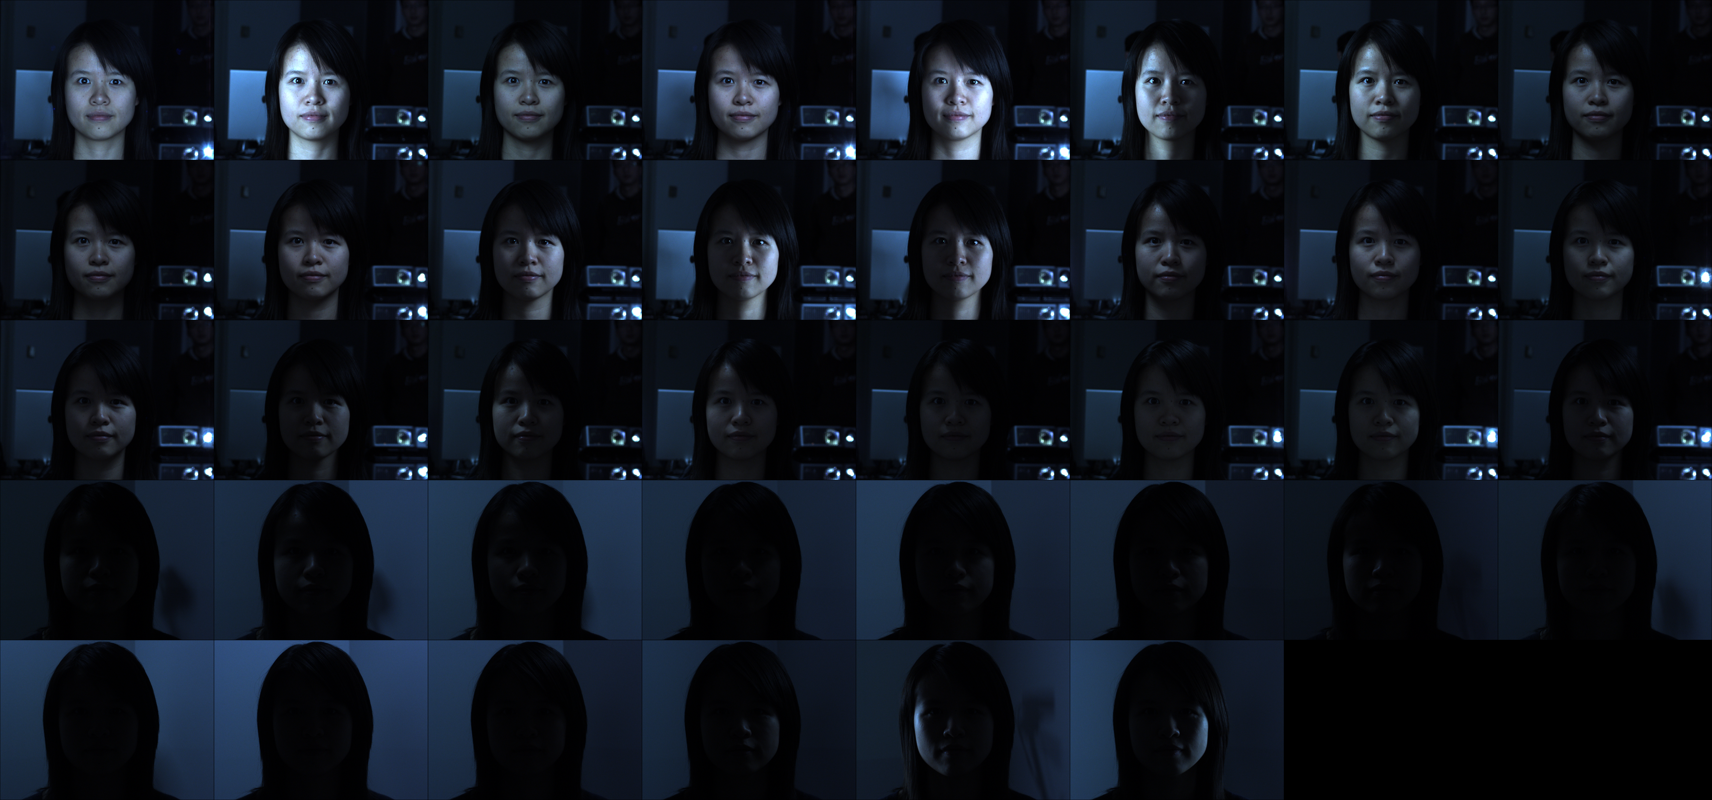
\includegraphics[width=\textwidth]{images/training_contact_sheet.png}
}

%\frame{\frametitle{Sample Training Images, Aligned and Cropped}
%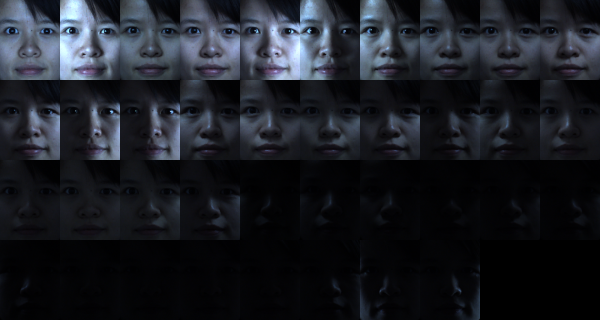
\includegraphics[width=\textwidth]{images/training_contact_sheet_cropped.png}
%}

